\chapter{Implementierung}
In diesem Kapitel wird die Implementierung der Methode näher erläutert. Bei der Implementierung werden alle Konzepte aus dem
Kapitel Konzeption angewendet.

% \section{Spiel-Datensatz}
% Für die Erstellung des Spiel-Datensatzes würde die Bibliothek ``Matplotlib''\footnote{https://matplotlib.org/} verwendet.

% \begin{lstlisting}[caption={Klasse Agent - Tensorflow Graph}, captionpos=b, label={lst:tf_graph_save}]
%   COLORS = [(236, 245, 66), (141, 245, 66), (245, 69, 66)]

%   for i in range(RANGE):
%     image = Image.new('RGB', (32, 32), 'black')
%     idx = np.random.randint(3)
%     x1 = np.random.randint(32)
%     y1 = np.random.randint(32)
%     x2 = np.random.randint(32)
%     y2 = np.random.randint(32)
  
%     draw = ImageDraw.Draw(image)
%     draw.rectangle((x1, y1, x2, y2), fill=COLORS[idx])
% \end{lstlisting}

\section{Binning}
Das Binning ist eine wichtige Komponente der Methode, dass mit Hilfe der ``numpy'' Bibliothek implementiert wurde. Als erstes wird 
anhand der Anzahl von Bins ($n\_bins$) die Breite ($B$) und Höhe ($H$) des \gls{grid}s, das auf der Abbildung \ref{image:bins} zu sehen ist,
mit Hilfe der Wurzel berechnet. Es wird angenommen dass $B = H$.
Nachdem die Breite des \gls{grid}s berechnet wurde, wird der Intervall von $[0, 1]$ in $B$ gleich große Intervalle aufgeteilt. Als nächstes
wird mit Hilfe der \textit{digitize} Funktion, der Intervall Index der jeweiligen $a, b$ Farbkanal Wert von jedem Pixel kalkuliert. 
Abschließend werden beide Indices zu einem Bin Index auf dem \gls{grid} umgewandelt. Der Output ist ein kodiertes Bild mit einem Bin Index per Pixel.
\\

\begin{listing}[H]
  \begin{minted}{python}
    # a, b sind die Koordinaten der Farbkanäle auf dem Grid
    def calculate_bin(a, b, width):
      return (width * b) + a
  
    def encode_bins(ab_image, n_bins):
      B = np.sqrt(n_bins).astype(int)
  
      # Intervall in gleich große Intervalle aufteilen
      interval = np.linspace(0, 1, B+1)
  
      # Indices für jeweils a, b Kanäle berechnen
      indices = np.digitize(ab_image, interval) - 1
  
      # Bin Index berechnen
      bins = np.vectorize(calculate_bin)(indices[:,:,0], indices[:,:,1], B)
  
      return bins
  \end{minted}
  \captionof{lstlisting}{Binning eines normalisierten Lab Bildes}
\end{listing}

\section{Datensätze}
Die Datensätze werden mit Hilfe der ``torchvision'' Bibliothek von PyTorch importiert und transformiert. Für das Importieren wurde eine
``ImageFolder'' implementiert, der die Bilder importiert, transformiert, normalisiert und in Bins kodiert. Der Output von den ``ImageFolder''
sind das Graustufenbild, das Bild mit den ``ab'' Farbkanäle und das in Bins kodierte Bild.

Mit Hilfe eines ``DataLoaders'' werden die Datensätze in Batches aufgeteilt und gemischt.

\section{Netzwerkarchitektur}
Für dieser Arbeit wurden 2 U-Nets mit verschiedene Größen verwendet. Ein U-Net für $ 32 \times 32 $ Bilder und ein U-Net für $ 128 \times 128 $ 
Bilder. Außerdem wurde das U-Net für $ 32 \times 32 $ Bilder angepasst damit es mit ein MSE Loss verwendet werden kann. Bei der Anpassung wurde
der Output Volumen zu $ W_{Input} \times H_{Input} \times 2 $ geändert, wobei das Netzwerk direkt die Werte für die ``ab'' Farbkanäle vorhersagt.
Bei der Verwendung von einem MSE Loss wird Binning nicht verwendet.

\subsection{ConvBlock}
Das Kernstück eines U-Nets ist der sogenannte ConvBlock. Ein ConvBlock beinhaltet zwei hintereinander geschaltete Blöcke, die wiederrum
aus einer Convolutional Layer mit $3 \times 3$ Filtern und Stride 1, gefolgt von ReLU und Batch Normalisation bestehen. 
Die Convolutional Layers verwenden Padding um die Dimensionen von dem Input nicht zu verändern. Die Layers wurden mit den PyTorch 
Klassen \textit{Conv2d}, \textit{BatchNorm2d} und die Funktion \textit{relu} implementiert.

\begin{figure}[H]
  \centering
  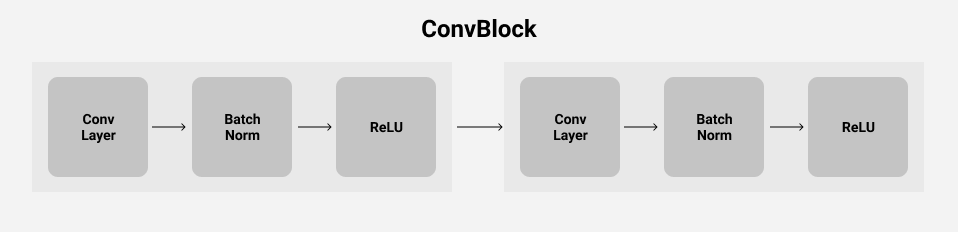
\includegraphics[width=1\textwidth]{resources/networks/convblock.png}
  \caption{
  ConvBlock
  }
  \label{image:convBlock}
\end{figure}

\subsection{U-Net}
Das U-Net für $32 \times 32$ Bilder besteht aus einem Encoder mit drei ConvBlocks. Die ersten zwei ConvBlocks werden von einem Pooling Layer
mit einem $2 \times 2$ Filter und Stride 2 gefolgt, um die Dimensionen zu halbieren. 
Der erste ConvBlock beinhaltet 16 Filter die nach jedem Pooling Layer verdoppelt werden. Die Dimensionen von den Feature Maps in der letzte
Layer des Encoders beträgt $8 \times 8 \times 64$. Der Decoder besteht aus zwei Transposed Convolutions mit $3 \times 3$ Filtern, Stride 2 und 
Padding 1 die die Dimensionen von den Feature Maps verdoppeln. Die Transposed Convolutions werden jeweils von einem ConvBlock gefolgt, das die
Anzahl der Filter halbiert. Das letzte Layer ist eine Convolutional Layer mit $1 \times 1$ Filtern, Stride 1 und Padding 0, das die 
Wahrscheinlichkeitsverteilung pro Pixel generiert. Die ersten zwei ConvBlocks aus dem Decoder werden jeweils mit den 2 Transposed Convolutions
aus dem Decoder konkateniert.
% \section{Beispiel Unterkapitel}
% TODO